Lorsqu'un langage régulier $L$, représenté par un automate $A_O$ tel que $L(A_O)=L$, est donné à l'oracle d'équivalence, il doit se prononcer sur $L=AL(F)$. Cependant, il ne possède pas d'automate pour $AL(F)$ qui est justement le langage recherché. Il doit alors se prononcer sur l'égalité en se basant uniquement sur $F$.

Comme expliqué dans l'introduction du chapitre, c'est impossible de façon générale. Cependant, en supposant que $AL(F)$ est régulier, il est possible de contourner le problème pour répondre à la question de sécurité.

Contrairement à la version originale de l'algorithme d'Angluin qui a deux possibilités (équivalence ou contre-exemple), celle-ci en a trois. L'oracle peut répondre soit que $AL(F)$ est sécurisé, soit qu'il ne l'est pas, soit que $L$ est différent de $AL(F)$ avec un contre-exemple.


\subsection*{$L$ est-il un point fixe de $\mathcal{F}$ ?}

Cette question se base sur la proprité de $\mathcal{F}$ disant que $\mathcal{F}(AL(F))=AL(F)$ ; que c'est une point fixe. Si $L$ n'est pas un point fixe, il n'a alors aucune chance d'être $AL(F)$. Les trois cas de la section \ref{ss:extension} donnent les différents détails.

Ceux-ci mentionnent trois possibilités :
\begin{itemize}
  \item On peut directement retourner un contre-exemple
  \item $L=AL(F)$ et la sécurité peut être calculée
  \item $L$ est une surapproximation de $AL(F)$. A ce moment, il faut se poser les deux autres questions pour pouvoir continuer à rafiner la compréhension de la relaiton entre $L$ et $AL(F)$.
\end{itemize}

\subsection*{$L$ intersecte-t-il avec une région à risque ?}

En visualisant $L$ comme étant un super-ensemble de $AL(F)$ et la région à risque comme un ensemble, il est possible de se représenter les différentes situations envisageables.

\begin{figure}[H]

  \colorlet{circle edge}{black}
  \colorlet{circle area}{blue!20}
  \colorlet{circle darker}{blue!40}
  \tikzset{filled/.style={fill=circle area, draw=circle edge},
    outline/.style={draw=circle edge}}

  \def\circleL{ (0,0) circle (1.5cm) node[right=0.8cm]  {$L$}}
  \def\circleAL{(-0.15,-0.3) circle (1cm) node {$AL(F)$}}

 \centering
 \begin{subfigure}{0.33\textwidth}
  \centering
  \def\circleUS{(0,2.8) circle (1cm) node[text width=1.5cm,align=center]  {Région à risque}}
  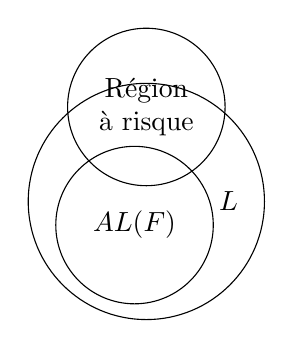
\begin{tikzpicture}
   \draw[outline]\circleL;
   \draw[outline]\circleAL;
   \draw[outline]\circleUS;
  \end{tikzpicture}
  \caption{Pas d'intersection}
 \end{subfigure}%
 \begin{subfigure}{0.33\textwidth}
  \centering
  \def\circleUS{(0,2.2) circle (1cm) node[text width=1.5cm,align=center]  {Région à risque}}
  \vspace{0.6cm}
  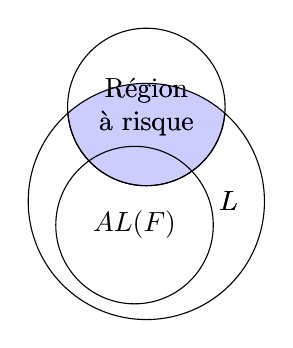
\begin{tikzpicture}
    \begin{scope}
        \clip \circleL;
        \fill[filled] \circleUS;
    \end{scope}
    \draw[outline]\circleL;
    \draw[outline]\circleAL;
    \draw[outline]\circleUS;
  \end{tikzpicture}
  \caption{Intersection avec $L$ seulement}
 \end{subfigure}
 \begin{subfigure}{0.33\textwidth}
   \centering
   \def\circleUS{(0,1.2) circle (1cm) node[text width=1.5cm,align=center]  {Région à risque}}
   \vspace{1.6cm}
   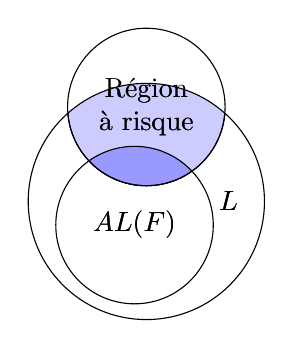
\begin{tikzpicture}
     \begin{scope}
         \clip \circleL;
         \fill[filled] \circleUS;
     \end{scope}
     \begin{scope}
         \clip \circleAL;
         \fill[filled, fill=circle darker] \circleUS;
     \end{scope}
     \draw[outline]\circleL;
     \draw[outline]\circleAL;
     \draw[outline]\circleUS;
   \end{tikzpicture}
  \caption{Intersection avec $AL(F)$}
 \end{subfigure}
 \caption{$L$, $AL(F)$ et la région à risque}\label{fig:inter}
\end{figure}

Pour savoir si nous sommes dans le scénario (a), (b) ou (c) de la figure \ref{fig:inter}, deux tests sont à effectuer.

Premièrement, vérifier si $\mathcal{W}(L)$ est vide ou non. S'il est vide, nous sommes dans le scénario (a) et il est possible d'annoncer avec certitude que $F$ est sécurisé.

\subsection*{Le chemin vers l'état à risque est-il valide ?}

Si la réponse à la question précédente est oui, sommes-nous dans le scénario (b) ou (c) ?
Considérons un des éléments de $\mathcal{W}(L)$. Demandons à l'oracle d'appartenance si ce mot appartient également à $AL(F)$.

Si ce n'est pas le cas, c'est que $L\neq AL(F)$ et que l'algorithme d'Angluin peut continuer grâce au contre-exemple fourni. Ici, il peut s'agir soit d'un scénario (b) soit d'un scénario (c) puisqu'un autre mot de $\mathcal{W}(L)$ pourrait appartenir à $AL(F)$. Améliorer l'approximation d'$AL(F)$ permet justement de mieux discriminer ces deux scénarios sans devoir consulter la totalité de $\mathcal{W}(L)$.

Si par contre le mot étudié appartient aussi à $AL(F)$, on a un mot étant à la fois dans $AL(F)$ et dans la région à risque. $F$ est déclaré à risque et le mot est retourné comme contre-exemple. Il s'agit du scénario (c).
